\documentclass{article}

\usepackage[a4paper, margin=0.8in]{geometry}
\usepackage{amsmath}
\usepackage{amssymb}
\usepackage{graphicx}
\usepackage{listings}
\usepackage{xcolor}
\usepackage{float}
\usepackage{placeins}
\usepackage{tikz}

\title{\hspace*{1.5cm}\textbf{EE 341: Communication Systems \newline Assignment 2}}
\author{G\ Raviteja (23110120) \ Govindu Vignesh (23110122)}
\date{}

\lstset{
    language=Matlab,
    basicstyle=\ttfamily\small,
    keywordstyle=\color{blue},
    commentstyle=\color{green!60!black},
    breaklines=true
}
\setlength{\abovedisplayskip}{8pt}
\setlength{\belowdisplayskip}{8pt}

\begin{document}

\maketitle

\section*{Submission Checklist}
\begin{itemize}
\item[$\rightarrow$] Theory derivations, assumptions, and interpretations are included.
\item[$\rightarrow$] Reproducible code files:
\begin{itemize}
\item \texttt{solve\_q1\_quantizer.m}
\item \texttt{solve\_q2\_radar.m}
\item \texttt{run\_all.m}
\end{itemize}
\item[$\rightarrow$] Figures and summary files are generated directly in the main assignment folder.
\item[$\rightarrow$] Numerical summaries are saved as \texttt{q1\_summary.mat} and \texttt{q2\_summary.mat}, and also printed in MATLAB Command Window.
\end{itemize}

This report is written in a theory-first manner. For each part, we first explain the communication-system intuition, then present the mathematical model, and finally connect the equations to what is expected in the generated plots/results. This mirrors practical engineering workflow: model the physics/statistics, design the receiver/quantizer structure, and then verify with data.

\section{Q1. Uniform Quantizer Design for 5G OFDM Signals}

The OFDM sample amplitude is modeled as a Gaussian random variable:
\begin{equation*}
X \sim \mathcal{N}(0,\sigma^2), \qquad
f_X(x)=\frac{1}{\sqrt{2\pi}\sigma}e^{-x^2/(2\sigma^2)}.
\end{equation*}

For an 8-bit uniform quantizer with clipping at $\pm V_{\max}$ and loading factor
\begin{equation*}
\gamma = \frac{V_{\max}}{\sigma},
\end{equation*}
we balance two effects:
\begin{itemize}
\item[$\rightarrow$] granular noise (inside clipping range),
\item[$\rightarrow$] overload noise (tails beyond clipping range).
\end{itemize}

Intuition: the OFDM waveform is a sum of many independently modulated subcarriers. By central-limit behavior, the time-domain sample histogram becomes close to Gaussian. This means low-amplitude samples are very common, while large peaks are rare but important. If the quantizer range is too narrow, rare peaks are clipped hard and create large error energy. If range is too wide, clipping reduces but quantization steps become coarse for the majority of samples near zero. Therefore, the best design must trade these two error mechanisms.

\subsection*{Q1.1 Theory: Granular and Overload Noise}

For a uniform quantizer with decision boundaries $\{b_k\}$ and reproduction levels $\{q_k\}$,
the exact granular distortion inside the operating range is
\begin{equation*}
P_{q,\text{gran}} = \sum_k \int_{b_k}^{b_{k+1}} (x-q_k)^2 f_X(x)\,dx.
\end{equation*}

This expression says: for each quantization cell, we weight squared quantization error by the probability of landing in that cell, then sum over all cells.

For a mid-tread uniform quantizer, this exact sum-of-integrals is the rigorous model. In practice, for high-resolution operation, the error within each cell is approximately uniform over $[-\Delta/2,\Delta/2]$, giving per-cell error variance $\Delta^2/12$. This approximation is very accurate when $\Delta$ is small relative to local signal variation scale.

The overload distortion is caused by clipping beyond $\pm V_{\max}$:
\begin{equation*}
P_{q,\text{ol}} = \int_{V_{\max}}^{\infty}(x-V_{\max})^2f_X(x)\,dx
+\int_{-\infty}^{-V_{\max}}(x+V_{\max})^2f_X(x)\,dx.
\end{equation*}

Using symmetry:
\begin{equation*}
P_{q,\text{ol}} = 2\int_{V_{\max}}^{\infty}(x-V_{\max})^2f_X(x)\,dx.
\end{equation*}

Define
\begin{equation*}
\phi(\gamma)=\frac{1}{\sqrt{2\pi}}e^{-\gamma^2/2},
\qquad
Q(\gamma)=\int_{\gamma}^{\infty}\phi(u)\,du.
\end{equation*}
Then
\begin{equation*}
P_{q,\text{ol}} = 2\sigma^2\left[(1+\gamma^2)Q(\gamma)-\gamma\phi(\gamma)\right].
\end{equation*}

Sketch of reduction: set $x=\sigma u$, use $V_{\max}=\gamma\sigma$, and expand $(u-\gamma)^2=u^2-2\gamma u+\gamma^2$. The three Gaussian tail integrals reduce to standard identities involving $Q(\gamma)$ and $\phi(\gamma)$.

Using standard Gaussian identities,
\begin{equation*}
\int_{\gamma}^{\infty}\phi(u)du = Q(\gamma),
\qquad
\int_{\gamma}^{\infty}u\phi(u)du = \phi(\gamma),
\qquad
\int_{\gamma}^{\infty}u^2\phi(u)du = Q(\gamma)+\gamma\phi(\gamma),
\end{equation*}
the overload integral simplifies directly to the compact expression used above.

For an 8-bit quantizer, the step size is
\begin{equation*}
\Delta = \frac{2V_{\max}}{2^B-1}, \qquad B=8.
\end{equation*}
Using the high-resolution approximation, the granular noise becomes
\begin{equation*}
P_{q,\text{gran}} \approx \frac{\Delta^2}{12}\,\Pr(|X|\leq V_{\max})
=\frac{\Delta^2}{12}\left(1-2Q(\gamma)\right),
\end{equation*}
which captures that only non-clipped samples contribute to granular distortion.

Total noise power:
\begin{equation*}
P_{q,\text{tot}} = P_{q,\text{gran}} + P_{q,\text{ol}}.
\end{equation*}

The corresponding theoretical SQNR is
\begin{equation*}
\text{SQNR}_{\text{th}}(\gamma)=10\log_{10}\left(\frac{\sigma^2}{P_{q,\text{tot}}(\gamma)}\right).
\end{equation*}
For normalized analysis ($\sigma^2=1$), this reduces to $10\log_{10}(1/P_{q,\text{tot}})$.

Hence, small $\gamma$ gives strong clipping (large overload noise), while large $\gamma$ increases $\Delta$ (large granular noise). The optimum $\gamma$ is where this tradeoff is minimized.

Expected curve behavior:
\begin{itemize}
\item[$\rightarrow$] $P_{q,\text{ol}}$ decreases rapidly with $\gamma$ because Gaussian tails decay fast,
\item[$\rightarrow$] $P_{q,\text{gran}}$ generally increases with $\gamma$ since $\Delta \propto V_{\max}$,
\item[$\rightarrow$] total noise is U-shaped versus $\gamma$, producing a single practical optimum.
\end{itemize}

\subsection*{Q1.2 Numerical Sweep and Optimal Loading Factor}

We sweep $\gamma$ over the practical range and compute
\begin{equation*}
\gamma_{\text{opt}}=\arg\min_{\gamma} P_{q,\text{tot}}(\gamma).
\end{equation*}

From the script output,
\begin{equation*}
\gamma_{\text{opt,theory}} \approx 3.926,
\qquad
\text{SQNR}_{\text{opt,theory}} \approx 40.57\ \text{dB}.
\end{equation*}

This optimum is physically reasonable for an 8-bit quantizer under Gaussian excitation: clipping is controlled enough to avoid heavy tail loss, while the step size remains fine for the high-probability central region.

Design-logic interpretation:
\begin{itemize}
\item[$\rightarrow$] For $\gamma<\gamma_{\text{opt}}$, overload dominates and SQNR drops sharply.
\item[$\rightarrow$] Around $\gamma_{\text{opt}}$, overload and granular distortions are balanced.
\item[$\rightarrow$] For $\gamma>\gamma_{\text{opt}}$, clipping is negligible but coarse quantization dominates.
\end{itemize}

\begin{figure}[H]
\centering
\begin{minipage}{0.48\textwidth}
\centering
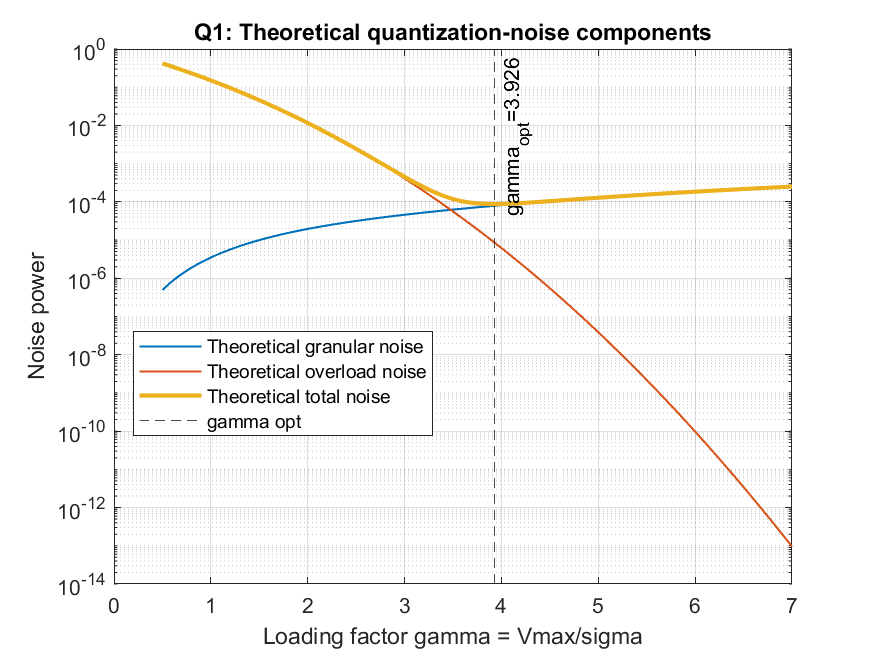
\includegraphics[width=\linewidth]{q1_theoretical_noise_vs_gamma.png}
\caption{Theoretical granular, overload, and total quantization noise versus $\gamma$.}
\end{minipage}
\hfill
\begin{minipage}{0.48\textwidth}
\centering
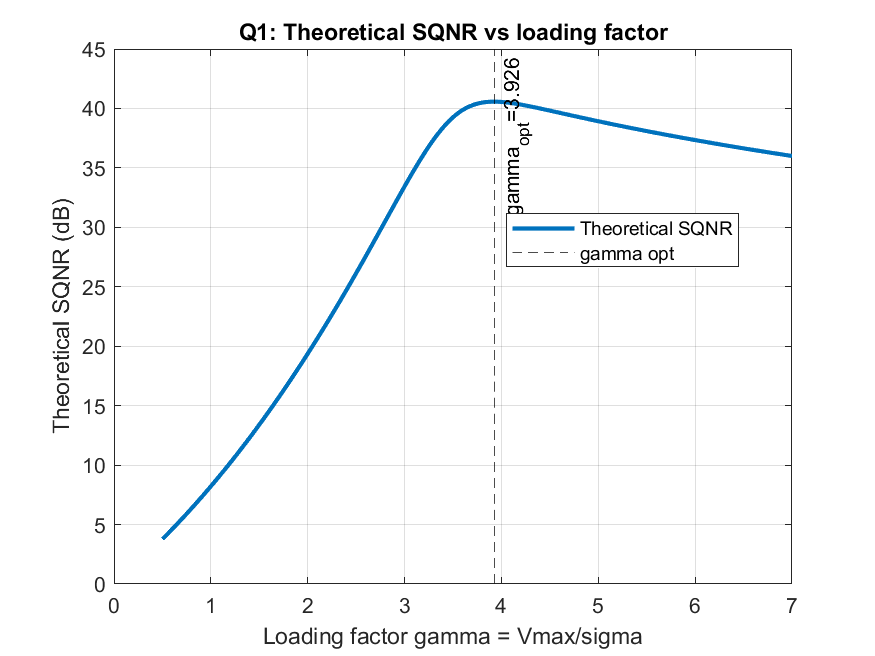
\includegraphics[width=\linewidth]{q1_theoretical_sqnr_vs_gamma.png}
\caption{Theoretical SQNR versus loading factor $\gamma$.}
\end{minipage}
\end{figure}

\FloatBarrier

\begin{figure}[H]
\centering
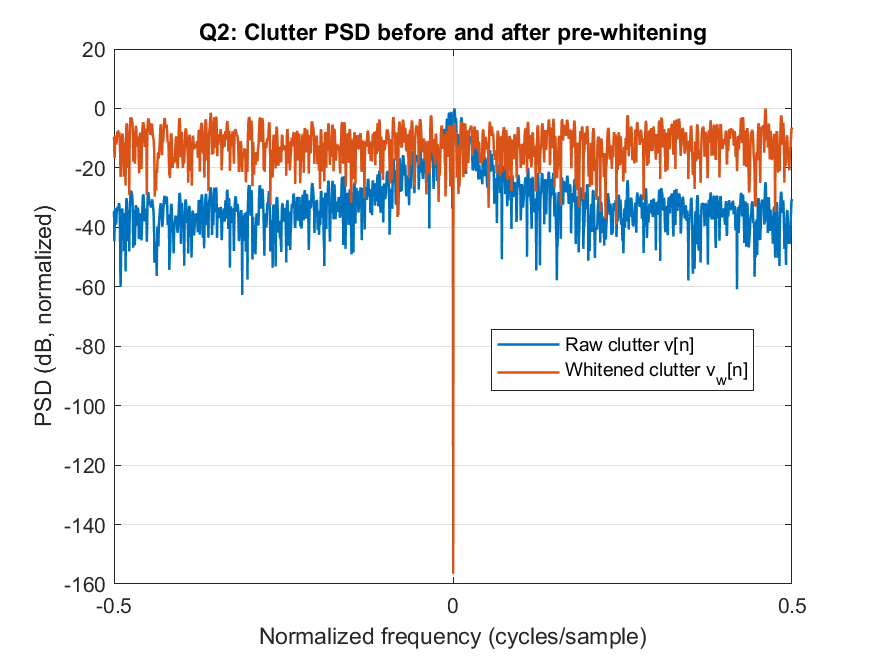
\includegraphics[width=0.75\textwidth]{q2_psd_before_after_whitening.png}
\caption{PSD comparison of clutter before and after pre-whitening.}
\end{figure}

\begin{figure}[H]
\centering
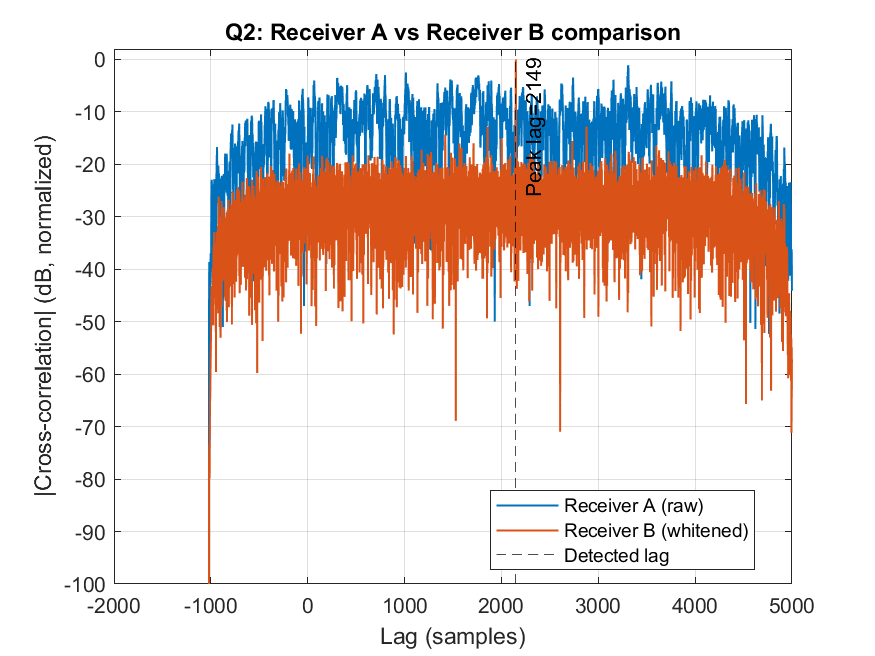
\includegraphics[width=0.75\textwidth]{q2_receivers_overlay_db.png}
\caption{Overlay comparison of Receiver A and Receiver B cross-correlation outputs in dB.}
\end{figure}

\FloatBarrier

\subsection*{Q1.3 Empirical SQNR with OFDM Dataset}

For the measured OFDM sequence, the empirical SQNR is computed as
\begin{equation*}
\text{SQNR}_{\text{emp}} = 10\log_{10}\left(\frac{\mathbb{E}[x^2]}{\mathbb{E}[(x-\hat{x})^2]}\right).
\end{equation*}

Method used in the experiment:
\begin{itemize}
\item[$\rightarrow$] load OFDM samples from \texttt{ofdm\_dataset.mat},
\item[$\rightarrow$] center data and estimate empirical $\sigma$,
\item[$\rightarrow$] quantize for each $\gamma$ using $V_{\max}=\gamma\sigma$,
\item[$\rightarrow$] compare empirical SQNR with the theoretical SQNR curve.
\end{itemize}

Why this comparison matters: the theoretical model assumes i.i.d. Gaussian samples and ideal quantization behavior. Real OFDM datasets can deviate due to finite packet length, pilot structure, windowing, and implementation details. The gap between curves is therefore a diagnostic, not just an error: it tells how realistic the Gaussian assumption is for the provided waveform.

Interpretation guideline:
\begin{itemize}
\item[$\rightarrow$] close agreement with theory indicates near-Gaussian amplitude statistics,
\item[$\rightarrow$] mismatch is expected from finite samples, imperfect Gaussianity, and practical OFDM waveform structure.
\end{itemize}

If the OFDM dataset is available, the script also writes:
\begin{itemize}
\item[$\rightarrow$] \texttt{q1\_theory\_vs\_empirical\_sqnr.png}
\end{itemize}

Using the provided dataset in this assignment, the empirical results are:
\begin{equation*}
\sigma_{\text{emp}} \approx 0.9999995,
\qquad
\gamma_{\text{opt,emp}} \approx 3.887,
\qquad
\text{SQNR}_{\text{opt,emp}} \approx 40.61\ \text{dB}.
\end{equation*}
These values are close to theoretical predictions, which supports the Gaussian approximation for the given OFDM samples.

A useful consistency check is the shift in optimum loading factor:
\begin{equation*}
\Delta\gamma = \gamma_{\text{opt,emp}}-\gamma_{\text{opt,theory}} \approx -0.039.
\end{equation*}
The small shift indicates mild practical non-idealities, but no major mismatch with the Gaussian-design assumption.

\begin{figure}[H]
\centering
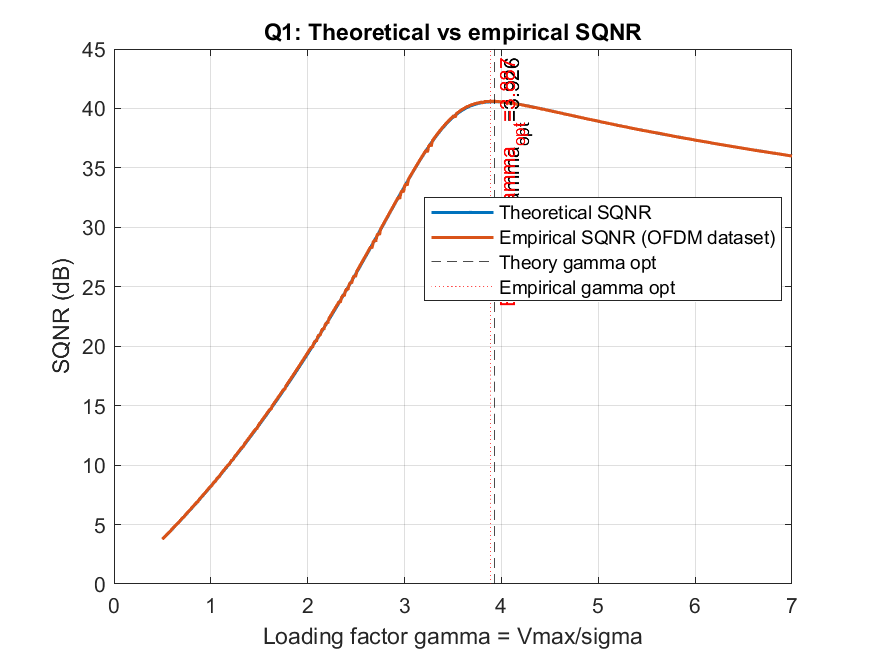
\includegraphics[width=0.65\textwidth]{q1_theory_vs_empirical_sqnr.png}
\caption{Theoretical and empirical SQNR comparison for the provided OFDM dataset.}
\end{figure}

\FloatBarrier

\section{Q2. Radar Detection in Colored Noise}

Given
\begin{equation*}
r[n] = s[n-n_0] + v[n],
\end{equation*}
where clutter is AR(1):
\begin{equation*}
v[n] = \alpha v[n-1] + w[n], \qquad w[n]\sim\mathcal{CN}(0,\sigma_w^2).
\end{equation*}

Intuition: the target echo is a delayed copy of known sequence $s[n]$, so correlation with $s[n]$ is the natural detector. However, clutter is not white; it has memory (strong low-frequency behavior). In such a case, naive matched filtering is no longer statistically optimal. Pre-whitening first removes clutter correlation so the subsequent correlation stage operates in a near-white-noise setting.

Hence, this problem is not only about implementing correlation, but about correcting the noise statistics first so that matched-filter optimality assumptions are restored.

\subsection*{Q2.1 Matched Filtering and Cross-Correlation Equivalence}
For a complex pulse, matched filter is
\begin{equation*}
h(t)=s^*(T-t).
\end{equation*}
Filter output:
\begin{equation*}
y(t)=\int r(\tau)h(t-\tau)\,d\tau
=\int r(\tau)s^*(T-(t-\tau))\,d\tau.
\end{equation*}
At $t=T$:
\begin{equation*}
y(T)=\int r(\tau)s^*(\tau)\,d\tau = R_{rs}(0).
\end{equation*}
Hence, matched-filter sampling at $T$ is equivalent to zero-lag cross-correlation.

This equivalence is the key reason cross-correlation is used directly in discrete implementations: it is exactly the matched-filter operation under standard conventions.

Equivalent discrete-time statement used in code:
\begin{equation*}
y[m] = \sum_n r[n]s^*[n-m] = (r \star s)[m].
\end{equation*}
Therefore the detection statistic is the cross-correlation peak over lag index $m$.

\subsection*{Q2.2 Estimation of $\alpha$ from Clutter-Only Samples}

From first 500 clutter-only samples,
\begin{equation*}
\hat{\alpha}=\arg\min_{\alpha}\sum_{n=1}^{N-1}|v[n]-\alpha v[n-1]|^2
=\frac{\sum_{n=1}^{N-1}v[n]v^*[n-1]}{\sum_{n=1}^{N-1}|v[n-1]|^2}.
\end{equation*}

This estimator is the complex least-squares/Yule-Walker form for AR(1), obtained by orthogonality of the residual with the regressor $v[n-1]$.

Detailed derivation idea:
\begin{itemize}
\item[$\rightarrow$] define cost $J(\alpha)=\sum |v[n]-\alpha v[n-1]|^2$,
\item[$\rightarrow$] take Wirtinger derivative with respect to $\alpha^*$,
\item[$\rightarrow$] set derivative to zero to obtain normal equation,
\item[$\rightarrow$] solve for ratio of lag-1 cross-term to lag-0 energy term.
\end{itemize}

Connection to Yule-Walker form:
\begin{equation*}
R_v[1] \approx \alpha R_v[0]
\quad\Rightarrow\quad
\hat{\alpha} \approx \frac{\hat{R}_v[1]}{\hat{R}_v[0]}.
\end{equation*}
This gives the same estimator and makes the statistical interpretation explicit.

\subsection*{Q2.3 FIR Pre-whitening Filter}

Using $v[n]-\alpha v[n-1]=w[n]$, choose
\begin{equation*}
H_w(z)=1-\hat{\alpha}z^{-1},
\end{equation*}
with impulse response
\begin{equation*}
h_w[n]=\delta[n]-\hat{\alpha}\delta[n-1].
\end{equation*}

This filter cancels the AR(1) memory term and leaves approximately white innovation noise, making matched filtering closer to the optimal AWGN condition.

Frequency-domain view: AR(1) clutter has PSD proportional to $1/|1-\alpha e^{-j\omega}|^2$. Multiplying by $|1-\hat{\alpha}e^{-j\omega}|^2$ flattens this spectrum when $\hat{\alpha}\approx\alpha$.

Therefore the whitened receiver effectively equalizes the clutter color before matched filtering, preventing low-frequency clutter dominance in the correlation output.

\subsection*{Q2.4 Receiver Architectures}
\begin{itemize}
\item[$\rightarrow$] Receiver A (Naive): cross-correlate raw $r[n]$ with raw $s[n]$.
\item[$\rightarrow$] Receiver B (Whitened): pre-whiten both $r[n]$ and $s[n]$, then cross-correlate.
\end{itemize}

Receiver B is expected to improve peak prominence and output SNR because strong low-frequency clutter energy is flattened before correlation.

Engineering expectation in plots:
\begin{itemize}
\item[$\rightarrow$] Receiver A: elevated background floor and weaker peak-to-floor contrast,
\item[$\rightarrow$] Receiver B: cleaner floor and sharper dominant peak near true delay.
\end{itemize}

Output SNR metric:
\begin{equation*}
\text{SNR}_{\text{out}} = 10\log_{10}
\left(\frac{|C[k_{\text{peak}}]|^2}{\mathbb{E}\{|C[k]|^2\,\text{outside}\,[k_{\text{peak}}-50,k_{\text{peak}}+50]\}}\right).
\end{equation*}

In implementation, the noise floor is estimated from all lags excluding a protection window around the peak ($\pm 50$ samples), so peak sidelobes do not bias the variance estimate.

\begin{figure}[H]
\centering
\begin{minipage}{0.48\textwidth}
\centering
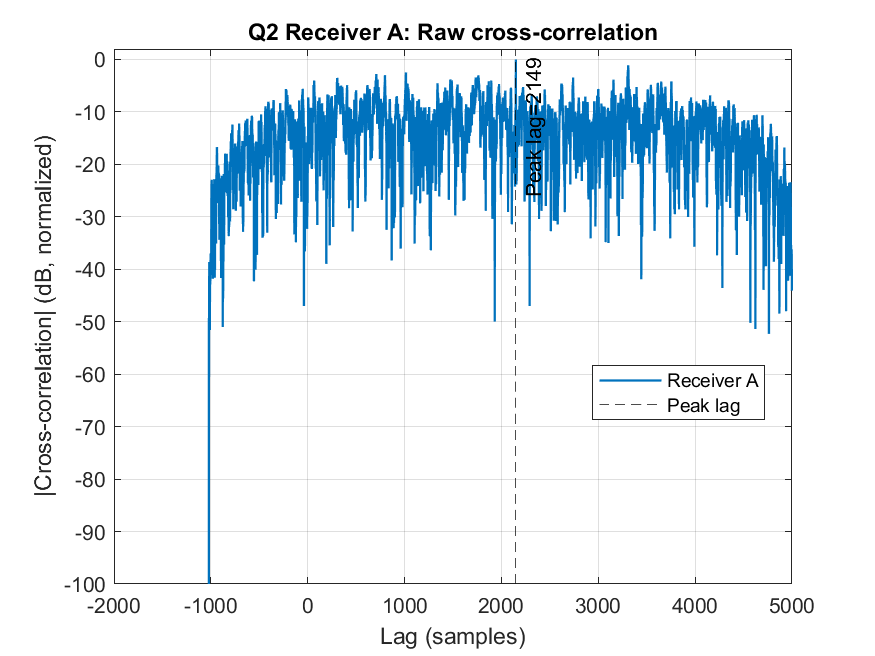
\includegraphics[width=\linewidth]{q2_receiver_A_xcorr_db.png}
\caption{Receiver A (naive) cross-correlation magnitude in dB.}
\end{minipage}
\hfill
\begin{minipage}{0.48\textwidth}
\centering
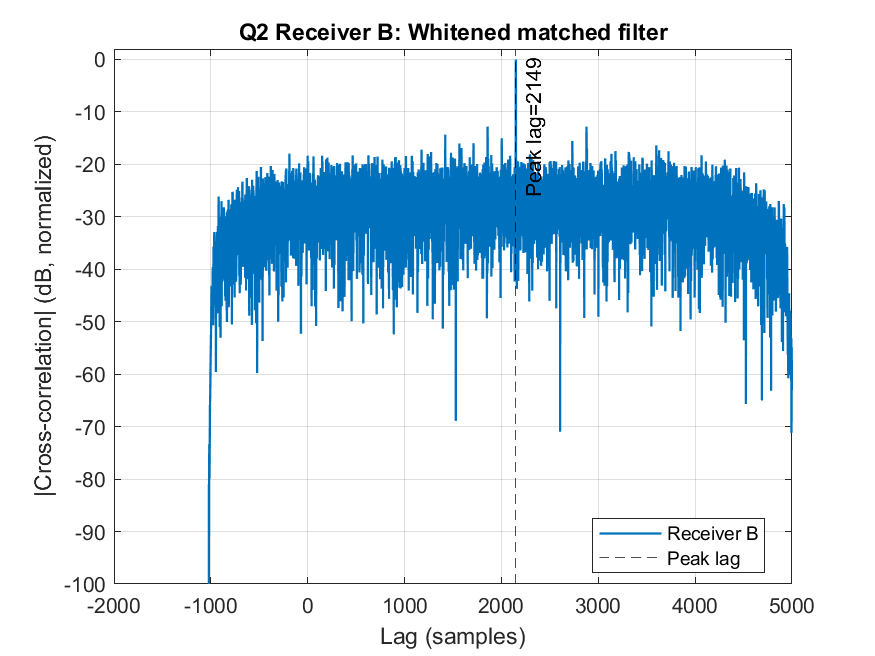
\includegraphics[width=\linewidth]{q2_receiver_B_xcorr_db.png}
\caption{Receiver B (whitened) cross-correlation magnitude in dB.}
\end{minipage}
\end{figure}

\FloatBarrier

If radar dataset is present, fill results from MATLAB output (Command Window) or \texttt{q2\_summary.mat}:
\begin{itemize}
\item[$\rightarrow$] Estimated AR parameter: $\hat{\alpha} \approx 0.94935 + j\,0.00303$.
\item[$\rightarrow$] Receiver A peak lag: $2149$ samples.
\item[$\rightarrow$] Receiver A output SNR: $13.77$ dB.
\item[$\rightarrow$] Receiver B peak lag: $2149$ samples.
\item[$\rightarrow$] Receiver B output SNR: $28.25$ dB.
\item[$\rightarrow$] SNR gain $(B-A)$: $14.48$ dB.
\end{itemize}

Quantitative conclusion from these values:
\begin{itemize}
\item[$\rightarrow$] both receivers localize the target at the same delay (lag $2149$), confirming no bias in target timing,
\item[$\rightarrow$] whitening improves output SNR by approximately $14.5$ dB, which is a major detection-performance gain,
\item[$\rightarrow$] the improvement magnitude is consistent with suppression of correlated clutter energy in the matched-filter output.
\end{itemize}

When both receivers are run on the same dataset, compare:
\begin{itemize}
\item[$\rightarrow$] peak lag consistency (target delay estimate),
\item[$\rightarrow$] output SNR improvement in Receiver B,
\item[$\rightarrow$] sidelobe/noise-floor suppression in dB plots.
\end{itemize}

If whitening is effective, peak lag should remain consistent while SNR increases. A large lag mismatch would indicate model mismatch, estimation error in $\hat{\alpha}$, or severe non-AR clutter components.

In our results, lag consistency is preserved and SNR increases strongly, so the AR(1)-based pre-whitening model is validated by the measured data.

The PSD figure gives direct physical evidence of this improvement: the raw clutter spectrum is strongly colored (low-frequency dominant), while the whitened clutter is considerably flatter. The overlay correlation figure further shows that whitening primarily lowers the effective noise floor while preserving the target lag location.

\section{Q3. Raised Cosine (RC) Filter}

In practical digital communication systems, pulse shaping is not only about bandwidth control, but also about controlling Inter-Symbol Interference (ISI). The raised-cosine (RC) spectrum is specifically designed so that, after matched filtering and symbol-rate sampling, neighboring symbols do not interfere. This is why RC filters are fundamental in modem design.

Given roll-off factor $\beta$ and symbol period $T$, the RC frequency response is
\begin{equation*}
H_{RC}(f)=
\begin{cases}
T, & |f|\le\dfrac{1-\beta}{2T},\\[4pt]
\dfrac{T}{2}\left[1+\cos\left(\dfrac{\pi T}{\beta}\left(|f|-\dfrac{1-\beta}{2T}\right)\right)\right], & \dfrac{1-\beta}{2T}<|f|\le\dfrac{1+\beta}{2T},\\[6pt]
0, & |f|>\dfrac{1+\beta}{2T}.
\end{cases}
\end{equation*}

Since $H_{RC}(f)$ is real and even, its impulse response is also real and can be obtained using
\begin{equation*}
h_{RC}(t)=\int_{-\infty}^{\infty}H_{RC}(f)e^{j2\pi ft}\,df
=2\int_0^{\infty}H_{RC}(f)\cos(2\pi ft)\,df.
\end{equation*}

To evaluate this integral, split the spectrum into two parts:
\begin{itemize}
\item[$\rightarrow$] flat passband contribution for $0\le f\le \dfrac{1-\beta}{2T}$,
\item[$\rightarrow$] cosine roll-off contribution for $\dfrac{1-\beta}{2T}<f\le \dfrac{1+\beta}{2T}$.
\end{itemize}

The passband integral gives the familiar sinc-type term, while the roll-off integral contributes a cosine-modulated correction that introduces the denominator $1-(2\beta t/T)^2$. After simplification, the closed-form RC impulse response is
\begin{equation*}
h_{RC}(t)=\frac{\sin(\pi t/T)}{\pi t/T}\cdot\frac{\cos(\pi\beta t/T)}{1-(2\beta t/T)^2}.
\end{equation*}

This is the standard result used in communication texts and software libraries.

\subsection*{Special Points and Continuity}
The formula above has removable singularities at specific time instants. Therefore we evaluate limits to obtain finite values:
\begin{equation*}
h_{RC}(0)=1,
\end{equation*}
and for $\beta\neq 0$,
\begin{equation*}
h_{RC}\left(\pm\frac{T}{2\beta}\right)=\frac{\beta}{2}\sin\left(\frac{\pi}{2\beta}\right).
\end{equation*}

These values are important in implementation because direct substitution in code can produce a division-by-zero warning if limits are not handled explicitly.

\subsection*{Nyquist ISI Interpretation}
The RC pulse satisfies the Nyquist zero-ISI condition:
\begin{equation*}
h_{RC}(nT)=
\begin{cases}
1, & n=0,\\
0, & n\in\mathbb{Z},\;n\neq 0.
\end{cases}
\end{equation*}
Hence, at ideal symbol-rate sampling instants, each symbol sees only its own pulse and no deterministic interference from neighboring symbols.

\subsection*{Role of Roll-Off Factor $\beta$}
The roll-off factor controls the bandwidth-time tradeoff:
\begin{itemize}
\item[$\rightarrow$] occupied (one-sided) baseband bandwidth is $\dfrac{1+\beta}{2T}$,
\item[$\rightarrow$] smaller $\beta$ gives tighter spectrum but longer time-domain ringing,
\item[$\rightarrow$] larger $\beta$ gives wider spectrum but faster decay in time.
\end{itemize}

So, $\beta$ is a system-level design knob: spectral efficiency pushes toward smaller $\beta$, while timing robustness and practical filter truncation push toward larger $\beta$.

Extreme cases:
\begin{itemize}
\item[$\rightarrow$] $\beta \to 0$: RC tends to the ideal sinc pulse (minimum bandwidth, maximum time spread),
\item[$\rightarrow$] $\beta \to 1$: widest transition band, smoother spectral edges, and better time localization.
\end{itemize}

\begin{figure}[H]
\centering
\begin{minipage}{0.48\textwidth}
\centering
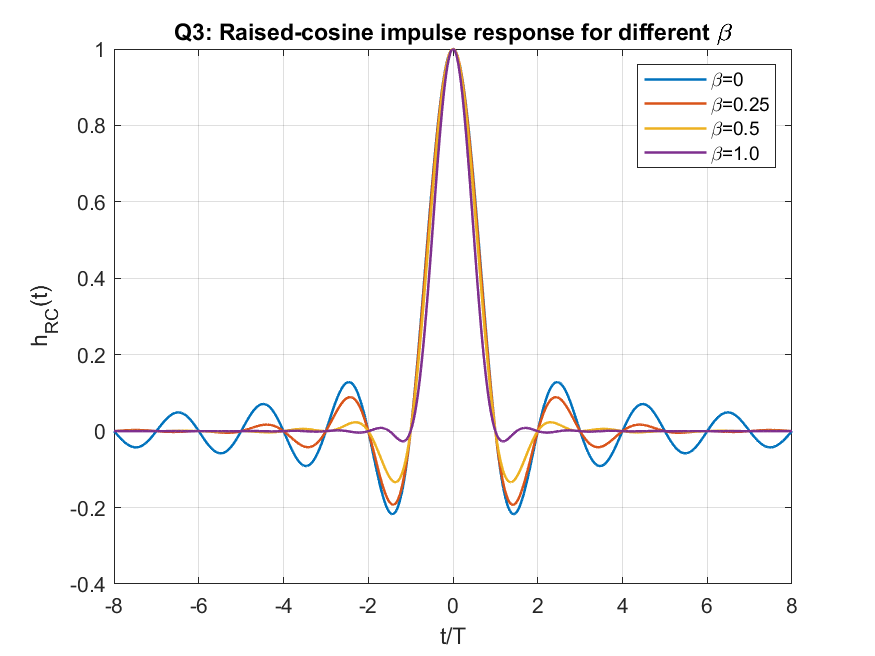
\includegraphics[width=\linewidth]{q3_rc_impulse_beta_comparison.png}
\caption{RC impulse responses for different roll-off factors $\beta$.}
\end{minipage}
\hfill
\begin{minipage}{0.48\textwidth}
\centering
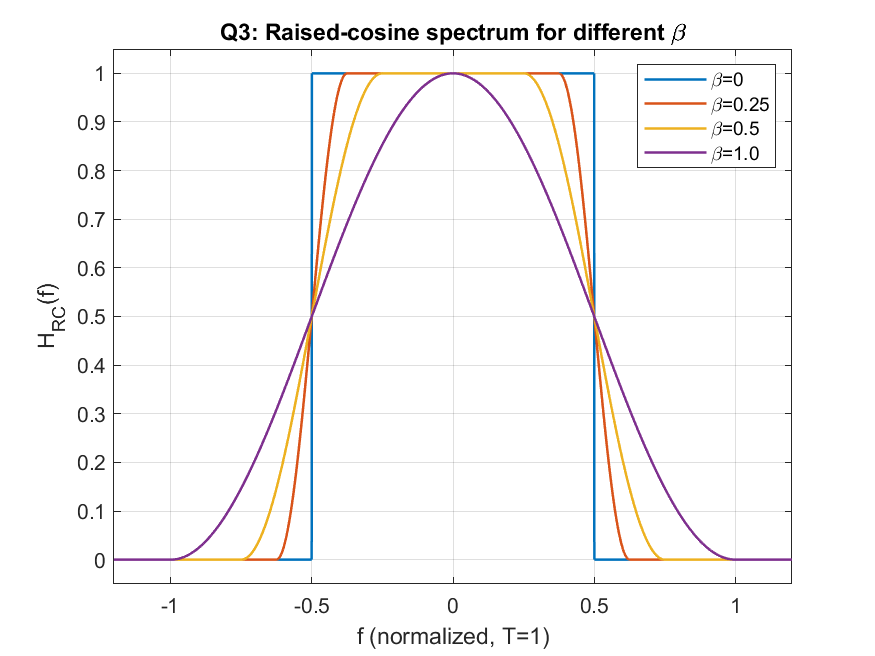
\includegraphics[width=\linewidth]{q3_rc_frequency_beta_comparison.png}
\caption{RC frequency responses for different roll-off factors $\beta$.}
\end{minipage}
\end{figure}

\FloatBarrier

From these plots, the design tradeoff is visually clear: smaller $\beta$ compresses bandwidth but increases time-domain ringing, while larger $\beta$ relaxes spectral compactness and yields faster temporal decay.

\section*{How to Reproduce Results}
Run from assignment folder:
\begin{lstlisting}
run('run_all.m')
\end{lstlisting}

Current workspace status:
\begin{itemize}
\item[$\rightarrow$] Q1 theoretical figures compile and generate correctly.
\item[$\rightarrow$] Q1 theory optimum values are verified: $\gamma_{\text{opt}}\approx 3.926$, SQNR $\approx 40.57$ dB.
\item[$\rightarrow$] Q1 empirical curve has been generated using \texttt{ofdm\_dataset.mat}.
\item[$\rightarrow$] Q2 final numeric outputs and plots have been generated using \texttt{cazac\_radar\_dataset.mat}.
\end{itemize}

\section*{Conclusion}
The assignment highlights a common communication-systems design pattern: statistical modeling and receiver/ADC structure must be co-designed. In Q1, the best loading factor appears from balancing two competing distortions rather than minimizing either one alone. In Q2, optimal detection in correlated clutter is achieved by transforming the noise statistics (whitening) before matched filtering. In Q3, raised-cosine design shows the fundamental time-frequency tradeoff in pulse shaping through $\beta$.

\end{document}
